\chapter{Combinaison de classifieurs}

\section{Combinaison par somme et produit de probabilités}

Afin d'améliorer les taux de reconnaissances obtenus par l'utilisation indépendante des deux classifieurs, il est possible de combiner les probabilités obtenues pour chaque classifieur afin d'obtenir un unique vecteur de probabilité d'appartenance. Deux méthodes de combinaison sont utilisées : la somme et la produit.\\

Soient pbelonging1 et pbelonging2 les probabilités d'appartenance respectivement obtenus pour les classifieurs 1 et 2. Les nouvelles probabilités, obtenues par combinaison en utilisant la somme et le produit, sont données de la façon suivante :

$$pbelongingsum(x/\omega_i) = pbelonging1(x/\omega_i) + pbelonging2(x/\omega_i)
pbelongingprod(x/\omega_i) = pbelonging1(x/\omega_i)pbelonging2(x/\omega_i)$$

avec x l'objet testé pour la classe d'appartenance \omega_i


\section{Critique des résultats obtenus}

\begin{figure}[h]
	\begin{center}
		\includegraphics{img/courbes taux fct d.png}
	\end{center}
	\caption{Comparaison des différents taux de reconnaissance en fonction du paramètre d}
\end{figure}
Rq : vert noir bleu superposés

\begin{figure}[h]
	\begin{center}
		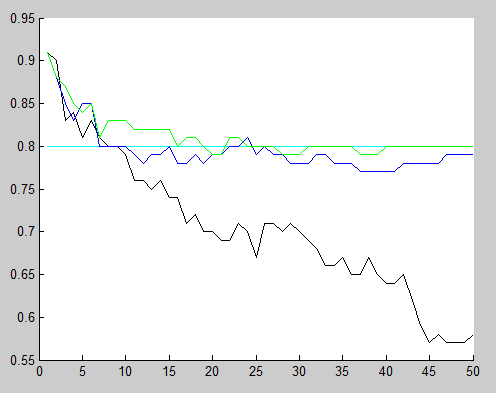
\includegraphics{img/courbes taux fct k.png}
	\end{center}
	\caption{Comparaison des différents taux de reconnaissance en fonction du paramètre k}
\end{figure}

\begin{figure}[h]
	\begin{center}
		\includegraphics{img/courbes taux fct mn.png}
	\end{center}
	\caption{Comparaison des différents taux de reconnaissance en fonction des paramètres m et n}
\end{figure}
Rq : vert noir et bleu superposés